\chapter{Conclusions and outlook}
\label{sec:conclusions1}


\section{Conclusions for ${\rm X \to qV~or~VV}$ analysis}

An inclusive sample of multijet events corresponding to an integrated
luminosity of \intlumi, collected in pp collisions at
$\sqrt{s}=8$\TeVcc with the CMS detector, is used to measure the
$\PW/\cPZ$-tagged dijet mass spectrum for the two leading jets,
produced within the pseudorapidity range $|{\eta}| < 2.5$ with a
separation in pseudorapidity of $|{\Delta\eta}| < 1.3$. The generic
multijet background is suppressed using jet-substructure tagging
techniques that identify vector bosons decaying into $\qqbarprime$ pairs
merged into a single jet. In particular, the invariant mass of pruned
jets and the $N$-subjettiness ratio $\tau_{21}$ of each jet are used
to reduce the initially overwhelming multijet background. The
remaining background is estimated through a fit to smooth analytic
functions. 

With no evidence for a peak on top of the smoothly falling
background, lower limits are set at the 95\% confidence level on
masses of excited quark resonances decaying into qW and qZ at 3.2 and
2.9 TeV, respectively. Randall--Sundrum gravitons \GRS decaying into
WW are excluded up to 1.2 TeV, and $\PWpr$ bosons decaying into
$\PW\cPZ$, for masses less than 1.7 TeV.  

For the first time mass
limits are set on $\PWpr\to \PW\cPZ$ and \GRS $\to \PW\PW$ in the
all-jets final state. 
%The mass limits on $q^*\to q\PW$, $q^*\to
%q\cPZ$, $\PWpr\to \PW\cPZ$, \GRS$\to \PW\PW$ are the most stringent
%to date.  
A model with a ``bulk'' graviton $\GBulk$ that decays into
WW or ZZ bosons is also studied, but no mass limits could be set due
to the small predicted cross sections.

\section{Conclusions for ${\rm X \to VH}$ analysis}
A search for a massive resonance decaying 
into a standard model-like Higgs boson and a W or Z boson is presented.
A data sample corresponding to an integrated luminosity of \intlumi
collected in proton-proton 
collisions at $\sqrt{s}=8$ TeV with the CMS detector
has been used to measure the W/Z and Higgs boson-tagged 
dijet mass spectra
using the two highest $\pt$ jets within the pseudorapidity range $|\eta| <
2.5$ and with pseudorapidity separation $|\Delta\eta| < 1.3$.  The QCD
background is suppressed using 
 jet substructure tagging techniques,
which identify boosted bosons decaying into hadrons.  In particular, 
the mass of pruned jets and the $N$-subjettiness ratios
$\tau_{21}$ and $\tau_{42}$, as well as b tagging applied to the subjets
of the Higgs boson jet, are used to discriminate
against the otherwise overwhelming QCD background.  The remaining QCD
background is estimated from a fit to the dijet mass distributions using a smooth function. 

We have searched for the signal as a peak on top of the smoothly
falling QCD background.  No significant signal is observed. 
In the HVT model B, 
a ${\rm Z'}$ is excluded in resonance mass intervals [1.0, 1.1] and 
[1.3, 1.5] TeV, while a ${\rm W'}$ is excluded in the interval [1.0, 1.6] TeV.  
A mass degenerate 
${\rm W'}$ plus ${\rm Z'}$ particle is excluded in the interval [1.0, 1.7] TeV.  

This is the first search for heavy resonances decaying into
a Higgs boson and a vector boson (W/Z) 
resulting in a hadronic final state,
as well as the first application of jet substructure techniques
to identify 
$\Hww$ decays of the Higgs boson at high Lorentz boost.

\section{Outlook}

The most recent ATLAS search on the VV analysis discovering a $\approx$3 sigma 
bump at $\approx$2 TeV, as shown in Figure~\ref{fig:atlasvv}. 
\begin{figure}[!htbp]
\centering
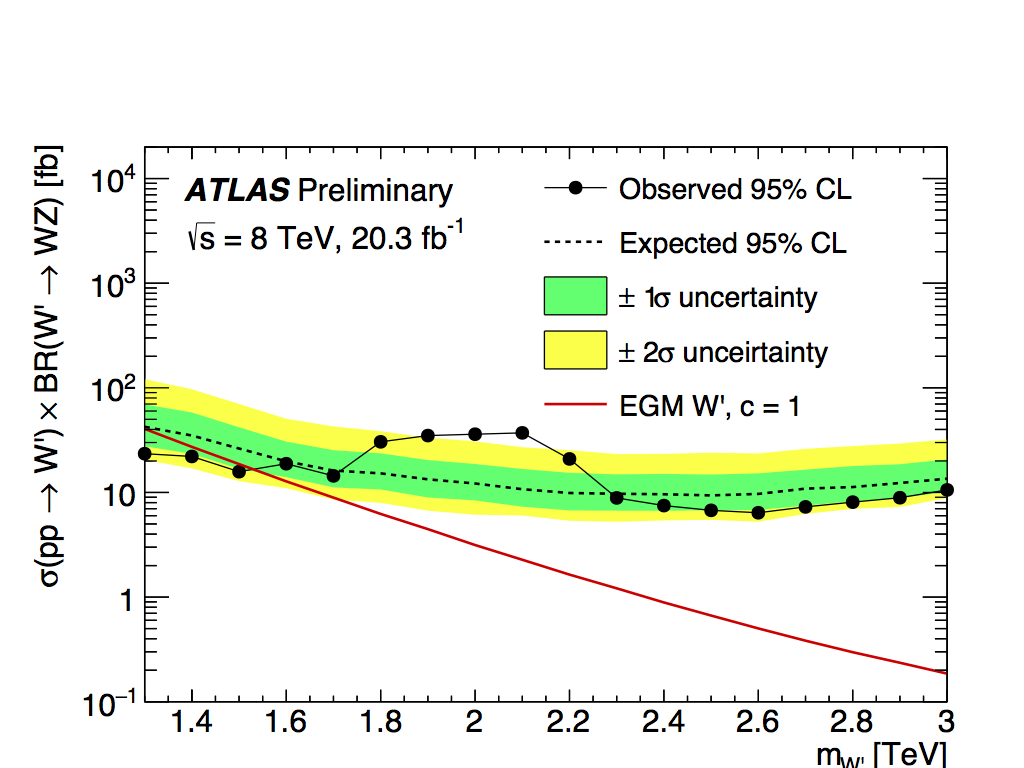
\includegraphics[width=.9\textwidth]{figures/atlas.png}
\caption{ATLAS results on the VV channel analysis.}
\label{fig:atlasvv}
\end{figure}
Similar effects were also observed in CMS VV analysis, but with a smaller excess of 1.3 sigma at
$\approx$1.9 TeV.  In 2015, the center collision energy of LHC will reach 13 TeV, with a high 
luminosity. With more events, we could verify the bump as of just a statistical fluctuation or a 
big discovery. 
 
The discovery of the Higgs boson was a tremendous vindication of the hard work of thousands of physicists and engineers for the past 30 years. However, it is just a beginning, for $\approx$96\% of 
the universe (dark matter, dark energy) is beyond the standard model and our current understanding. 
With the help of LHC, together we will go far. 




 

